% Options for packages loaded elsewhere
\PassOptionsToPackage{unicode}{hyperref}
\PassOptionsToPackage{hyphens}{url}
\documentclass[twocolumn
]{article}
\usepackage{xcolor}
\usepackage{amsmath,amssymb}
\setcounter{secnumdepth}{-\maxdimen} % remove section numbering
\usepackage{iftex}
\ifPDFTeX
  \usepackage[T1]{fontenc}
  \usepackage[utf8]{inputenc}
  \usepackage{textcomp} % provide euro and other symbols
\else % if luatex or xetex
  \usepackage{unicode-math} % this also loads fontspec
  \defaultfontfeatures{Scale=MatchLowercase}
  \defaultfontfeatures[\rmfamily]{Ligatures=TeX,Scale=1}
\fi
\usepackage{lmodern}
\ifPDFTeX\else
  % xetex/luatex font selection
\fi
% Use upquote if available, for straight quotes in verbatim environments
\IfFileExists{upquote.sty}{\usepackage{upquote}}{}
\IfFileExists{microtype.sty}{% use microtype if available
  \usepackage[]{microtype}
  \UseMicrotypeSet[protrusion]{basicmath} % disable protrusion for tt fonts
}{}
\makeatletter
\@ifundefined{KOMAClassName}{% if non-KOMA class
  \IfFileExists{parskip.sty}{%
    \usepackage{parskip}
  }{% else
    \setlength{\parindent}{0pt}
    \setlength{\parskip}{6pt plus 2pt minus 1pt}}
}{% if KOMA class
  \KOMAoptions{parskip=half}}
\makeatother
\usepackage{graphicx}
\makeatletter
\newsavebox\pandoc@box
\newcommand*\pandocbounded[1]{% scales image to fit in text height/width
  \sbox\pandoc@box{#1}%
  \Gscale@div\@tempa{\textheight}{\dimexpr\ht\pandoc@box+\dp\pandoc@box\relax}%
  \Gscale@div\@tempb{\linewidth}{\wd\pandoc@box}%
  \ifdim\@tempb\p@<\@tempa\p@\let\@tempa\@tempb\fi% select the smaller of both
  \ifdim\@tempa\p@<\p@\scalebox{\@tempa}{\usebox\pandoc@box}%
  \else\usebox{\pandoc@box}%
  \fi%
}
% Set default figure placement to htbp
\def\fps@figure{htbp}
\makeatother
\setlength{\emergencystretch}{3em} % prevent overfull lines
\providecommand{\tightlist}{%
  \setlength{\itemsep}{0pt}\setlength{\parskip}{0pt}}
\usepackage{bookmark}
\IfFileExists{xurl.sty}{\usepackage{xurl}}{} % add URL line breaks if available
\urlstyle{same}
\hypersetup{
  hidelinks,
  pdfcreator={LaTeX via pandoc}}

\author{}
\date{}

\begin{document}

\subsection{CS431 HW 1 Findings}
The following is a study of parallelizing the integration method of
calculating pi. In an attempt to lower the runtime of the code below,
the researcher implemented three parallel adaptations.

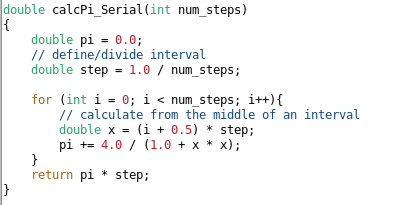
\includegraphics[width=3.11809in,height=1.62649in]{./media/image1.png}

The researchers first attempt used "pragma omp parallel" for above the
for loop and an atomic lock on pi within the loop.

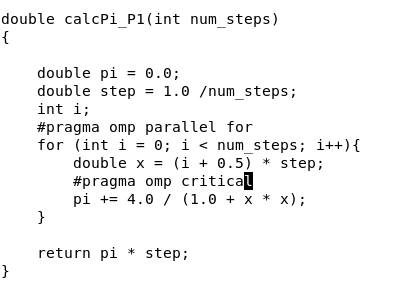
\includegraphics[width=3.15696in,height=2.35193in]{./media/image2.png}

In initial testing on a four core virtual linux debian instance, this
parallel version performed worse than the serial version. As the
researcher increased the number of steps, the program scaled quite
poorly and started to take upwards of ten seconds to execute while the
serial version never took more than one and a half seconds.

Assuming the critical section was a bottleneck, the researcher swapped
these for a locking system. This did not improve the performance to any
noticeable degree.

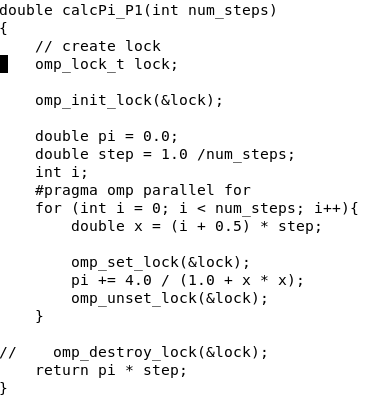
\includegraphics[width=2.18787in,height=1.94576in]{./media/image3.png}

Abandoning manual locking altogether proved to be the most efficient
solution of those attempted. By declaring the iterator i as private and
including the reduction flag for the variable pi, the researcher found a
meaningful performance increase.

Across twenty tests of the integration techniques with num\_steps =
100000000, the median for the serial implementation was 1.46192 seconds
and a mean of 1.46252. The median for the final parallel version was
0.0167111 and mean of 0.0174611 seconds.

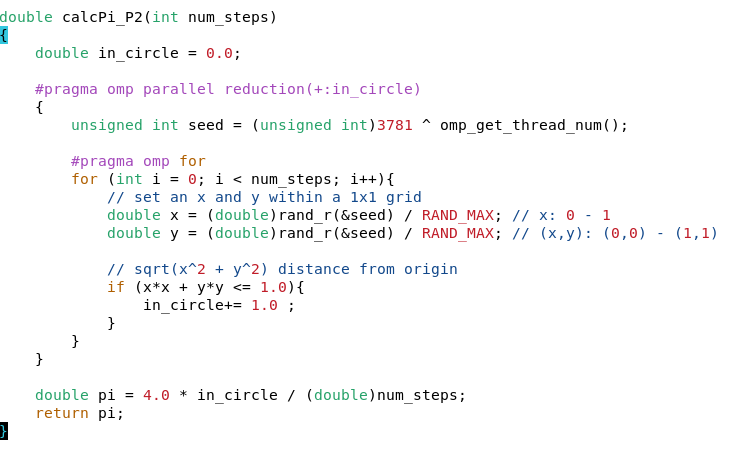
\includegraphics[width=2.64601in,height=1.58945in]{./media/image4.png}

The screenshot above shows the Monte-Carlo implementation in parallel.
Splitting the fork from the for loop allowed a unique seed to be
generated for each core. Although this method was faster than serial
integration, the resulting pi value was less accurate than integration.

The median runtime of 20 runs and num\_steps = 100000000 was 0.0188663
seconds and mean 0.0188613 seconds.

\end{document}
